% Drawing 69/06-8 -- folder 69, batch 06, archive page 117 (PDF page 118).
% Transcription: un triangle de sommets $u$ (en bas à gauche), $v$ (en bas à droite) et $w$ (en haut) ; de chaque sommet partent quatre paires d'arêtes, dessinées comme des pointes effilées ouvertes vers l'extérieur. Autour de $u$ : les paires $(\alpha_i, \alpha'_i)$, groupées par accolades en $a_1, \dots, a_4$ ; autour de $v$ : les paires $(\beta_i, \beta'_i)$, groupées en $b_1, \dots, b_4$ ; autour de $w$ : les paires $(\gamma_i, \gamma'_i)$, groupées en $c_1, \dots, c_4$. Plusieurs étiquettes sont repassées
% Kind: triangle u v w with four pairs of edges at each vertex. Method 2 (schematic redraw from the facsimile). Status: partial.
% Notes: Triangle u (lower left), v (lower right), w (top), its vertices placed once; from each vertex four pairs of edges drawn as narrow spikes opening outwards (each pair closed by a short stroke), every edge drawn from the vertex itself: around u the pairs (alpha_i, alpha'_i) braced a_1 ... a_4, around v (beta_i, beta'_i) braced b_1 ... b_4, around w (gamma_i, gamma'_i) braced c_2, c_3 and a third letter at the right. Labels where they stand on the page. The two long crossing strokes are not drawn. Redrawn 2026-11-09 (issue 128). Overlay check 2026-11-13 (claude-opus-5-5, issue 147): the 300 dpi colour rendering of the 250 ppi scan laid under the redraw, rasterised from its TikZ (not compiled: no TeX in the session): the triangle, the twelve spikes and the labels lie on their ink within about 1 unit; nothing moved. Still differs: several labels are overwritten (gamma_1, gamma'_1, gamma_2 at the top, beta_2, beta'_2 at the right) and are placed at their readable position; the braces are given by their letters only; the letter of the brace at the upper right, set c_4 in the redraw (it braces the gamma_4 spike), looks like c_1 on the scan (its index a single stroke with a small flag), and no fourth c letter can be found round w, so which of c_1 and c_4 stands there is a reading to check (the transcription names c_1 ... c_4).
% Coordinates: 1 unit = 1 mm = 1/100 of the crop width (bbox in page fractions: [0.08, 0.06, 0.5, 0.34]).
% Redrawn by Claude (claude-opus-5-5), issue #73, 2026-11-09; not checked by a human; not compiled (no TeX in the session).
% Checked by Claude (claude-opus-5-5) 2026-11-13 (issue #147): overlaid on the colour scan (250 ppi, rendered at 300 dpi) and corrected; not compiled (no TeX in the session), rasterised for the overlay by a Python reader of this TikZ. Status: partial.
% Rights: reproduces part of the work -- behind RENDER_TRANSCRIPTS, never published by itself.
\documentclass[tikz,border=3pt]{standalone}
\usepackage{amsmath,amssymb}
\usetikzlibrary{patterns,arrows.meta}
\tikzset{pencil/.style={black!45}, struck/.style={black!35}, mark/.style={circle,draw,inner sep=1.3pt}, pt/.style={circle,fill,inner sep=0.9pt}, opt/.style={circle,draw,fill=white,inner sep=1.1pt}}
\begin{document}
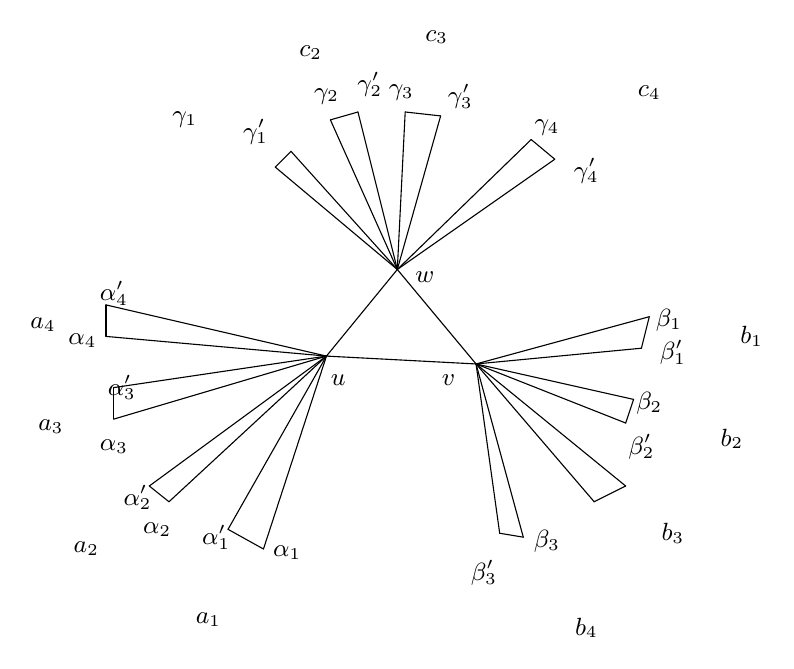
\begin{tikzpicture}[x=1mm,y=1mm,line cap=round,line join=round,font=\scriptsize]
\draw (46,-49.5) -- (65,-50.5) -- (55,-38.5) -- cycle;
\draw (55,-38.5) -- (39.5,-25.5);
\draw (55,-38.5) -- (41.5,-23.5);
\draw (39.5,-25.5) -- (41.5,-23.5);
\draw (55,-38.5) -- (46.5,-19.5);
\draw (55,-38.5) -- (50,-18.5);
\draw (46.5,-19.5) -- (50,-18.5);
\draw (55,-38.5) -- (56,-18.5);
\draw (55,-38.5) -- (60.5,-19);
\draw (56,-18.5) -- (60.5,-19);
\draw (55,-38.5) -- (72,-22);
\draw (55,-38.5) -- (75,-24.5);
\draw (72,-22) -- (75,-24.5);
\draw (46,-49.5) -- (18,-43);
\draw (46,-49.5) -- (18,-47);
\draw (18,-43) -- (18,-47);
\draw (46,-49.5) -- (19,-53.5);
\draw (46,-49.5) -- (19,-57.5);
\draw (19,-53.5) -- (19,-57.5);
\draw (46,-49.5) -- (23.5,-66);
\draw (46,-49.5) -- (26,-68);
\draw (23.5,-66) -- (26,-68);
\draw (46,-49.5) -- (33.5,-71.5);
\draw (46,-49.5) -- (38,-74);
\draw (33.5,-71.5) -- (38,-74);
\draw (65,-50.5) -- (87,-44.5);
\draw (65,-50.5) -- (86,-48.5);
\draw (87,-44.5) -- (86,-48.5);
\draw (65,-50.5) -- (85,-55);
\draw (65,-50.5) -- (84,-58);
\draw (85,-55) -- (84,-58);
\draw (65,-50.5) -- (84,-66);
\draw (65,-50.5) -- (80,-68);
\draw (84,-66) -- (80,-68);
\draw (65,-50.5) -- (68,-72);
\draw (65,-50.5) -- (71,-72.5);
\draw (68,-72) -- (71,-72.5);
\node[inner sep=1pt] at (58.5,-39.5) {\small $w$};
\node[inner sep=1pt] at (47.5,-52.5) {\small $u$};
\node[inner sep=1pt] at (61.5,-52.5) {\small $v$};
\node[inner sep=1pt] at (28,-19.5) {\small $\gamma_1$};
\node[inner sep=1pt] at (37,-21) {\small $\gamma'_1$};
\node[inner sep=1pt] at (46,-16.5) {\small $\gamma_2$};
\node[inner sep=1pt] at (51.5,-15) {\small $\gamma'_2$};
\node[inner sep=1pt] at (55.5,-16) {\small $\gamma_3$};
\node[inner sep=1pt] at (63,-16.5) {\small $\gamma'_3$};
\node[inner sep=1pt] at (74,-20.5) {\small $\gamma_4$};
\node[inner sep=1pt] at (79,-26) {\small $\gamma'_4$};
\node[inner sep=1pt] at (44,-11) {\small $c_2$};
\node[inner sep=1pt] at (60,-9) {\small $c_3$};
\node[inner sep=1pt] at (87,-16) {\small $c_4$};
\node[inner sep=1pt] at (19,-41.5) {\small $\alpha'_4$};
\node[inner sep=1pt] at (15,-47.5) {\small $\alpha_4$};
\node[inner sep=1pt] at (10,-45.5) {\small $a_4$};
\node[inner sep=1pt] at (20,-53.5) {\small $\alpha'_3$};
\node[inner sep=1pt] at (19,-61) {\small $\alpha_3$};
\node[inner sep=1pt] at (11,-58.5) {\small $a_3$};
\node[inner sep=1pt] at (22,-67.5) {\small $\alpha'_2$};
\node[inner sep=1pt] at (24.5,-71.5) {\small $\alpha_2$};
\node[inner sep=1pt] at (15.5,-74) {\small $a_2$};
\node[inner sep=1pt] at (32,-72.5) {\small $\alpha'_1$};
\node[inner sep=1pt] at (41,-74.5) {\small $\alpha_1$};
\node[inner sep=1pt] at (31,-83) {\small $a_1$};
\node[inner sep=1pt] at (89.5,-45) {\small $\beta_1$};
\node[inner sep=1pt] at (90,-49) {\small $\beta'_1$};
\node[inner sep=1pt] at (100,-47) {\small $b_1$};
\node[inner sep=1pt] at (87,-55.5) {\small $\beta_2$};
\node[inner sep=1pt] at (86,-61) {\small $\beta'_2$};
\node[inner sep=1pt] at (97.5,-60) {\small $b_2$};
\node[inner sep=1pt] at (90,-72) {\small $b_3$};
\node[inner sep=1pt] at (66,-77) {\small $\beta'_3$};
\node[inner sep=1pt] at (74,-73) {\small $\beta_3$};
\node[inner sep=1pt] at (79,-84) {\small $b_4$};
\end{tikzpicture}
\end{document}
